\documentclass[a4paper]{article}
\usepackage{amsfonts}
\usepackage{amsmath}
\usepackage{amssymb}
\usepackage{graphicx}
\usepackage{extarrows}

\newcommand{\integral}{\displaystyle\int}
\newcommand{\limit}{\lim\limits}

\begin{document}

\noindent \large Auteur: Seda Jusjajeva\\
\noindent \large Studierichting: Informatica\\
\noindent \large Oefeningenreeks 5F nr. 1.1\\

\medskip

\normalsize



$r = -\cos\theta$ \\

\begin{figure}[h]
\centering
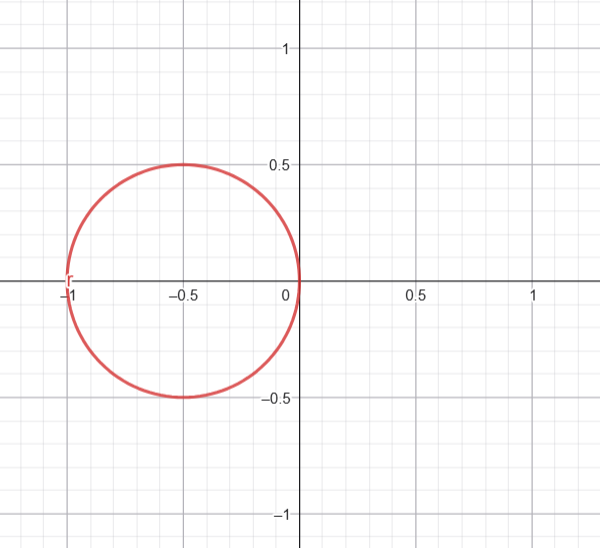
\includegraphics[width=8cm]{5F-1.1-seda.jusjajeva.INF.png}
\end{figure}

$S = 2\cdot\dfrac{1}{2}\integral^\pi_{\tfrac{\pi}{2}}\cos^2\theta d\theta$ \\

$\integral\cos^2\theta d\theta = \integral\dfrac{1 + \cos2\theta}{2}d\theta = \dfrac{1}{2}\integral d\theta + \dfrac{1}{2}\integral\cos2\theta d\theta =\dfrac{\theta}{2} + \dfrac{\sin2\theta}{4} + c$ \\

$\Rightarrow S = \left[\dfrac{\theta}{2} + \dfrac{\sin(2\theta)}{4}\right]_{\tfrac{\pi}{2}}^{\pi} = \dfrac{\pi}{2} + \dfrac{\sin(2\pi)}{2} - \left(\dfrac{\pi}{4} + \dfrac{\sin(\pi)}{2}\right) = \dfrac{\pi}{2} - \dfrac{\pi}{4} = \dfrac{\pi}{4}$\\




\begin{thebibliography}{999}
%\bibitem{a} Referentie
\end{thebibliography}
\end{document}